\subsection{Data Collection}
% WAITING: Get participant statistics from Chad
We collected data for 24 participants, via an EEG monitor equipped with 64 sensors (ActiCHamp, Revision 2, Brainproducts GmbH, Munich, Germany). Two mastoid sensors were dedicated as reference electrodes. Another electrode was used as the ground, leaving 61 total signal electrodes. Collection was performed in a sound-dampened room with participants facing a 19" LCD screen and interacting with the experiment using a button controller (VPixx, Vision Science Solutions, Quebec, Canada). The task was written in MATLAB (Version 8.6, Mathworks, Natick, U.S.A.) using the Psychophysics Toolbox extension~\cite{brainard1997psychophysics}.

\begin{figure}[t]
  \centering
  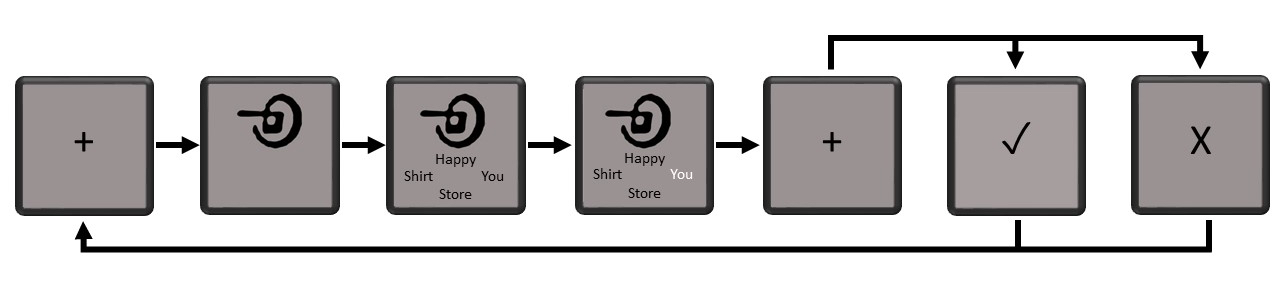
\includegraphics[width=\linewidth]{figures/experiment}
  \caption{The experimental paradigm. Participants were required to learn a mapping of symbols to English words through trial and error. This simulates a language learning task.}
  \label{fig:experiment}
\end{figure}

Participants viewed a series of symbols from the Tamil and Manipuri alphabets, which were assigned to a random English word (consistent across all participants, but having no relationship to the meaning of the Tamil or Manipuri words).  Participants were presented with a symbol, and asked to select the correct word from four options. The participant received visual feedback about their response: correct (``\CheckmarkBold'') or incorrect (``X''). Figure \ref{fig:experiment} illustrates a single trial of the paradigm. We hypothesized that as participants learned the mapping of symbols--to--words, they would also assign semantic meaning to each symbol. This simulates learning a language through a trial and error mechanism. Our task used a 1--to--1 mapping for symbols--to--words over a very small subset of English (60 words total), which is not representative of learning a complete language, but will allow us to detect the process of learning the symbol--to--word mapping.
  
To facilitate learning, symbols were selected from a set that grew as the experiment progressed. During the first block, participants were presented with six symbols (representing three pronouns, three verbs). In subsequent blocks, three new symbols (and thus three new words) were added. There were a total of 19 blocks, and 60 total symbols learned. Throughout the experiment, each of the participants viewed a random number of trials (ranging from 0--20, denoted as $n_t$) for each of the 60 symbols. Within the set of 60, three symbols corresponded to pronouns, three to verbs, and 54 to nouns. After the first block, the order in which symbols were added was randomly determined, so that no two participants viewed the noun symbols in the same order. These three words were randomly paired with three previously learned words so that each block cycled through six words.\reminder{Chad question: that last sentence seems out of place, what three words are you referring to?} 
  
The stimuli were displayed on a gray background.  Each trial begins with a black fixation cross for 700 to 1000 ms, followed by a symbol written in black, 4.5 cm\textsuperscript{2} in size. The symbol presented was randomly selected from the list of six for the block. After 500 ms, four black English words appeared in the arrangement of a fixation cross (top, bottom, right, left) below the symbol. One of the choices was the correct answer, and the three distractor words (incorrect answers) were randomly chosen from the remaining five words. The assignment of words to the four locations was randomly determined. Participants were instructed to respond by pressing one of the buttons on the RESPONSEPixx controller, which also has response buttons arranged in a cross. Once a participant made a selection, the selected word turned white for 500 ms, the screen changed to a fixation for 700 to 1000 ms, and a feedback stimulus appeared for one second (``\CheckmarkBold'' or ``X''). If a selection was not made within two seconds, an exclamation mark would appear to signify that they took too long to respond. Ten words were presented sequentially at a time \reminder{Chad question: what happens after the 10 words?} and participants continued until receiving 90\% or higher accuracy \reminder{Chad question: this doesn't make sense, 90\% over a set of 10?  We know some participants didn't do this well}. 
  
To further facilitate the transfer of meaning to symbols, participants also viewed three word sentences containing one pronoun, one verb, and one noun (e.g., \emph{I am happy}). Three sentences were interleaved with word learning phase described above. In these phases, participants saw one word at a time for one second each, separated by a fixation cross for 700 to 1000 ms, which was followed by four multiple choice answers as to indicate what the sentence had said. For the purposes of our study, the sentence trials were discarded. The participants each saw approximately 500 exposures, including sentences, with breaks provided.
